\section{Introduction}

% --------------------------------------------------------------------------------------------------------------
\begin{frame}
\frametitle{Pagerank}
\begin{figure}
	\centering
	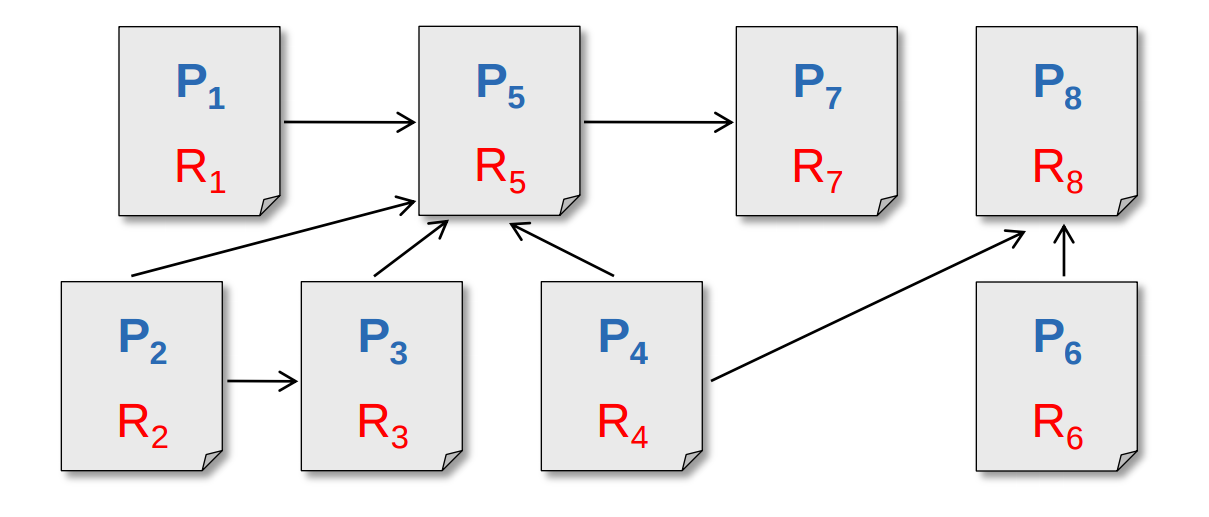
\includegraphics[width=0.8\textwidth]{pagerank1.png}
	\caption{PageRank example 1 \cite{prsigner}}
\end{figure}
\begin{itemize}
  \item A page has a high PageRank $R$ if
  \begin{itemize}
    \item there are many pages linking to it
    \item or, if there are some pages with a high PageRank
linking to it
  \end{itemize}
\end{itemize}
\end{frame}
% --------------------------------------------------------------------------------------------------------------

% --------------------------------------------------------------------------------------------------------------
\begin{frame}
\frametitle{Pagerank}

\begin{minipage}[l]{0.5\textwidth}
\textbf{$$ 
R(P_i)= \sum_{P_j \in B_i}\frac{R(P_j)}{L_j}
$$}
\begin{itemize}
  \item where
  \begin{itemize}
    \item $B_i$ is the set of pages that link to page $P_i$
    \item $L_j$ is the number of outgoing links for page $P_j$
linking to it
  \end{itemize}
\end{itemize}
\end{minipage}
\begin{minipage}[l]{0.49\textwidth}
\begin{figure}
	\centering
	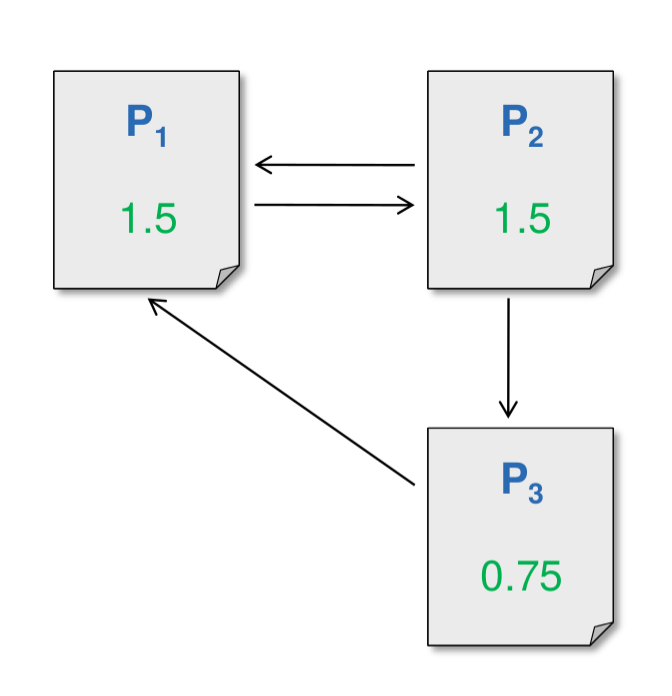
\includegraphics[width=\textwidth]{pagerank2.png}
	\caption{PageRank example 2 \cite{prsigner}}
\end{figure}
\end{minipage}

\end{frame}
% --------------------------------------------------------------------------------------------------------------

% --------------------------------------------------------------------------------------------------------------
\begin{frame}
\frametitle{Apache Flink}
Effiziente Implementierung relationaler Joins im Hadoop-Framework
\hspace{8pt}
\begin{itemize}
  \item 2 Verfahren
  \begin{itemize}
    \item Realisierung ohne Veränderung des Hadoop-Frameworks
    \item Erweiterung des Hadoop-Frameworks um einen
    Merge-Operator
  \end{itemize}
  \item Tests der Verfahren gegeneinander
\end{itemize}
\end{frame}
% --------------------------------------------------------------------------------------------------------------
